\documentclass[../../what-is-computer]{subfiles}
\begin{document}
        
    \subsection{Ancient calculators}

    So, essentially, what is a computer? And yes, there is a definition from Merriam-Webster dictionary in the first pages. \emph{But what does computer do, in its essence?}.
    Well, it \emph{computes}, duh. \emph{So, the computer is a buffed-up calculator? Well, it is an oversimplification, but not really untrue}. If a five-year old asked me
    what a computer is, I would definetely tell him, it is a calculator, but very powerful and calculating all sorts of stuff\footnote{I want to believe, that an explanation in 
    the previous section gave you a clue, how it transforms all the stuff into numbers.}. \par

    I want to devote this section to a brief historical overview of computers. Please, keep in mind, that it is a \emph{vast} topic. However, there are some moments in the very
    beginning of computer history, that interests me the most, regarding this essay. Since this essay puts the programming perspective into focus, I want to explore 
    a bit, how did the programming started. \par

    But where should we start? Well, since computer was oversimplied to rather big calculator, I suggest we start with the calculators.\par

    The first attempts to help us count things are ancient. The first thing coming to mind is an \emph{abacus} or \emph{abaci} for plural. We don't know exacly when or
    where it emerged\footnote{\href{https://en.wikipedia.org/wiki/Abacus}{https://en.wikipedia.org/wiki/Abacus}}. However, we do know, that many cultures used some form
    of abacus or counting frame for calculating purposes. The principle behind those auxiliary devices they used is virtually the same in every cultures, despite the 
    details being a little bit different. We have multiple names for different types of abaci in different
    cultures\footnote{\href{https://en.wikipedia.org/wiki/Abacus}{https://en.wikipedia.org/wiki/Abacus}}:
    \begin{table}[h]
        \centering
        \begin{longtable} {p{0.15\textwidth}p{0.2\textwidth}p{0.2\textwidth}p{0.3\textwidth}}
            \toprule
            Original name & Transcription & Origin & Additional Info \\
            \toprule
            算盤 & suanpan & China & \\
            そろばん & soroban & Japan & Can be represented as `算盤' also \\
            주판 & jupan & Korea & Could also be called supan (수판), jusan (주산) \\
            nepohualtzintzin & & Aztec Culture & \\
            счеты & schoty & Russia & \\
            \bottomrule
            \caption{Abaci in different cultures}
            \end{longtable}
    \end{table}

    \newpage


    However, those are purely mechanical and manual devices, main principle of which is very similar to how we convert numbers to different bases. They still
    require us to `translate' our numbers to abacus system and, after we've done our math, translate them back. \par


    \begin{wrapfigure}{lh}{0.3\textwidth}
        \centering
        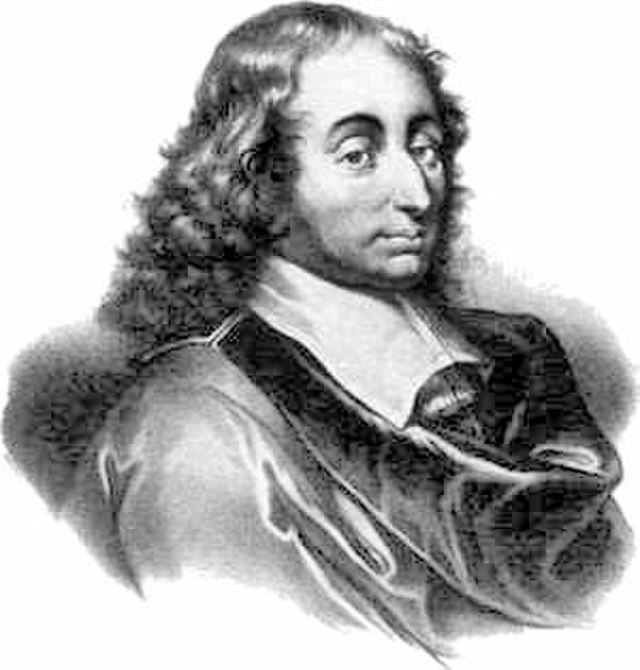
\includegraphics[scale=0.1]{images/persons/person_blaise_pascal.jpg}
        \caption{Blaise Pascal}
    \end{wrapfigure}

    The first succesful automation attempt is attributed to Blaise Pascal, with his \emph{Arithmetic Machine} which is also called a \emph{Pascaline}.
    It was designed and built between 1642 and 1644\footnote{\href{https://www.britannica.com/technology/Pascaline}{https://www.britannica.com/technology/Pascaline}}. 
    Pascaline could only add and subtract numbers, using rotational dials as an input.\par


    % \begin{wrapfigure}{r}{0.5\textwidth}
    %     \centering
    %     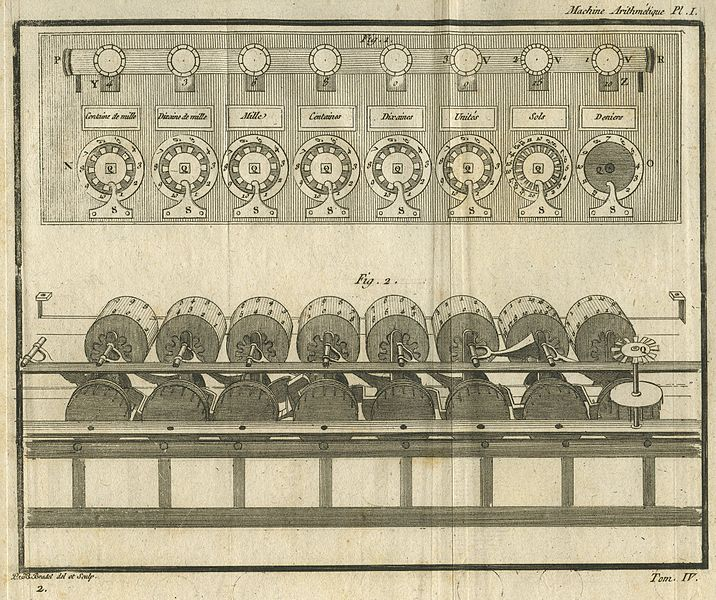
\includegraphics[scale=0.3]{images/devices/device_pascaline_scheme.jpg}
    %     \caption{Top view and overview of the mechanism}
    % \end{wrapfigure}

    There are several pascalines still intact nowadays, most of the remaining ones are in european museums. Being the first calculator isn't the only achievement
    of pascaline. Pascal was only 18 years old, when he started designing his machine, trying to help his father with accounting. He went through about 50 prototypes
    before settled on the final one. Later Pascal presented his machine to the public, and, eventually, to the King of France, receiving a royal privilege, which 
    was basically a patent in those days. And yes --- his father did use it in work afterwards \par


    Pascaline wasn't a computer, but it was first in many ways --- first calculator, which was afterwards commercialized, used in business and patented. Many of 
    subsequent attemps to farther automate calculations were directly inspired by Pascaline. \par

    \subsection{Luddites' nightmare}

    \begin{wrapfigure}{r}{0.3\textwidth}
        \centering
        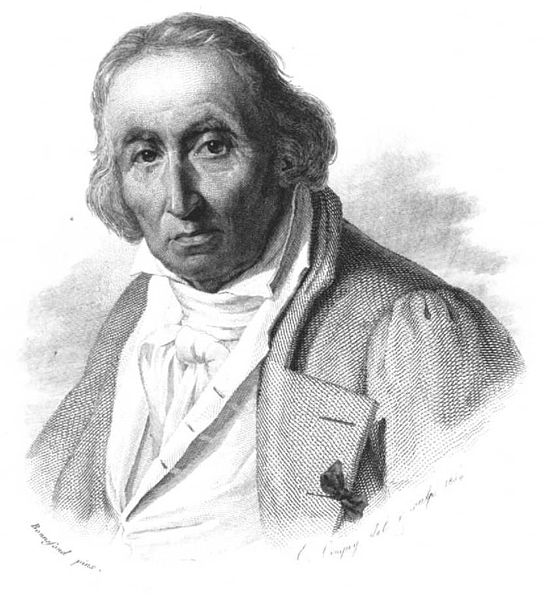
\includegraphics[scale=0.2]{images/persons/person_joseph_jacquard.jpg}
        \caption{Joseph Marie Jacquard}
    \end{wrapfigure}

    The next machine of our interest is not a computer either. It isn't even a calculator --- it's a loom. I cannot say much about weaving history, 
    but in computer history, it was indeed the most significant loom there is. In 1804 a french weaver and merchant, Joseph Marie Jacquard invented a \emph{Jacquard Machine}. \par

    Beginning of the 19\textsuperscript{th} century is pretty much a middle of industrial revolution. New fancy industrial looms are practically a 
    symbol of the new era. Industrial revolution changed our world forever, marking a \emph{transition from hand production methods to machines}.
    Despite Great Britain being the origin of the industrial revolution, it spread eventually over the continent, and afterwards, the world. 
    Industrial revolution eventually lead to the \emph{emergence of the capitalist economy}. In other words --- \emph{Industrial revolition was a big deal}. \par

    \begin{wrapfigure}{r}{0.5\textwidth}
        \centering
        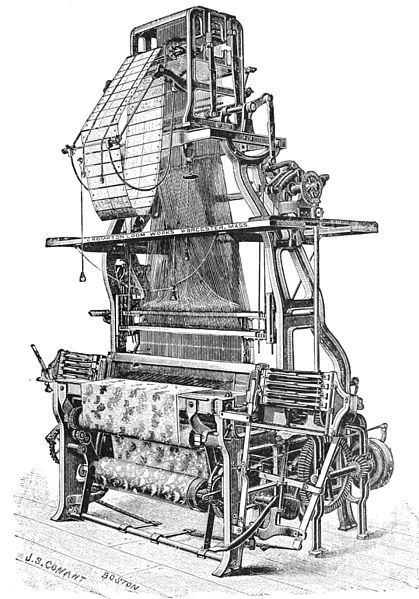
\includegraphics[scale=0.2]{images/devices/device_jacquard_loom.jpg}
        \caption{Jacquard Loom}
    \end{wrapfigure}

    So, amidst all this revolution going, we could see how a work, that was being done by 100 men before can be done by 10 men with machines. It was \emph{super effecient}.
    Inventors tried to find a way to increase production effeciency (and therefore revenue) by exploring technical capabilities of the machines they worked with. So 
    Joseph Jacquard invented his machine, which was basically an \emph{attachment to the industrial loom}. A loom with an attached machine was subsequently called
    \emph{Jacquard Loom}\footnote{Jacquard Loom is a general term, which does not describe any concrete loom, but rather any loom with the control 
    mechanism, allowing pattern weaving automation}. \par

    The main purpose of Jacquard's attachment was an \emph{pattern weaving automation}. It used a chain of special cards laced together in a continuous, looped sequence.
    Those cards will later be called \emph{punch cards}. Punch card is, essentially a card, with designated spaces for holes. Later, some designated space would be `punched'
    to produce a hole in area. Some spaces were omitted during `punching'. After `punching' those holes we would have a card, partially filled with holes. Jacquard Loom
    relies on a simple mechanical action of those cards. While continuously moving, those cards would move controlling rods of the loom, therefore affect knot being weaved. 
    If there was no hole in the area, rod will move since card will push it. If there was a hole, rod wouldn't move since it would go through hole. \par


    \begin{wrapfigure}{l}{0.5\textwidth}
        \centering
        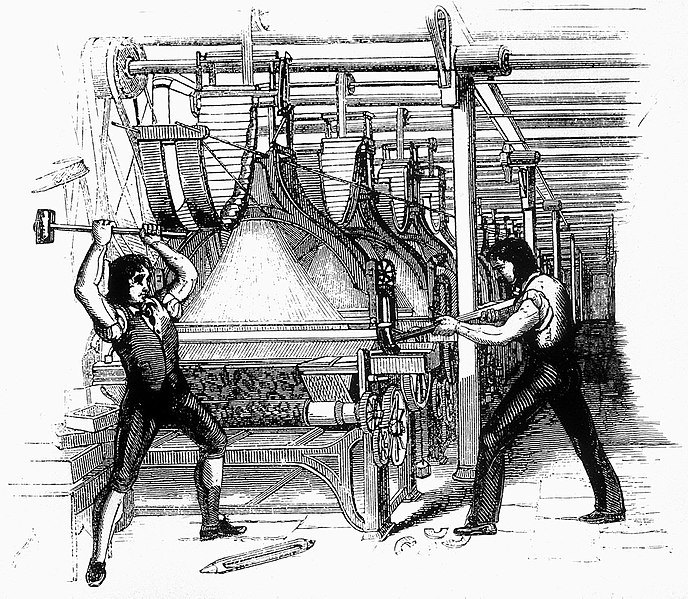
\includegraphics[scale=0.2]{images/misc/luddites.jpg}
        \caption{1844's depiction of Luddites destroying the loom}
    \end{wrapfigure}

    This machine would \emph{drastically} impact effeciency, since it was no longer required to be of high skill to weave complicate patterns. It, essentially, gave
    manufacturers ability to \emph{store design patterns and to reproduce them indefinitely}\footnote{At least until punch cards are in fine condition}. The man behind
    the punching process still needed to be trained and qualified, but to just reproduce a readily punched design wasn't much of an issue even to a low-skill worker.
    Just imagine a reaction from weavers, that used to work by hand. No surprise, that \emph{Luddites}\footnote{The term itself initially related to an organisation 
    of English textile workers. However, over time it has come to mean one opposed to new technologies in general}
    destroyed such machines to protest against their usage. \par

    \subsection{Steam, calculators and British Government}
    \begin{wrapfigure}{l}{0.3\textwidth}
        \centering
        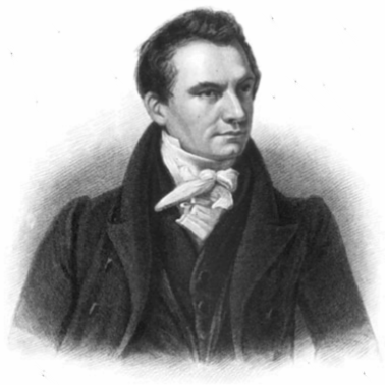
\includegraphics[scale=0.2]{images/persons/person_charles_babbage.png}
        \caption{Charles Babbage}
    \end{wrapfigure}

    Well, the idea of using automation in weaving patterns have touched deeply not only the Luddites, but also at least one mathematician, which was also a philosopher,
    inventor and mechanical engineer. It's just so happened this was also a man, who will be considered as the `father of the computer'\footnote{\href{https://cse.umn.edu/cbi/who-was-charles-babbage}
    {https://cse.umn.edu/cbi/who-was-charles-babbage}} by many. Some of his works even touched the subject of industrialization and economy, which influenced Karl 
    Marx\footnote{\href{https://projects.exeter.ac.uk/babbage/rosenb.html}{https://projects.exeter.ac.uk/babbage/rosenb.html}}. A man called Charles Babbage was deeply
    inspired by Joseph Jacquard's invention and intended to use his ingenious punch cards in his own machine. \par

    Charles Babbage was an inventor of 2 machines, that are of interest in this essay: \emph{Difference Engine} and \emph{Analytical Engine}. Both of these machines
    were not finished in his lifetime, unfortunately. Nonetheless, this heritage of 2 unfinished machines marked a signinificant point in history of computers. More 
    than that, \emph{those 2 machines gave an opportunity for the first ever programmer to become a first ever programmer}. \par

    \begin{wrapfigure}{r}{0.5\textwidth}
        \centering
        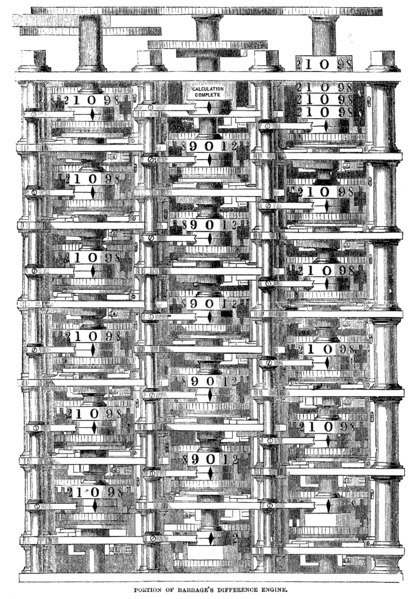
\includegraphics[scale=0.25]{images/devices/device_babbage_difference_engine.jpg}
        \caption{Part of Babbage's Difference Engine}
    \end{wrapfigure}


    The Difference Engine, essentially was a giant mechanical calculator, that was powered by steam and printed results of it's computations in a table. 
    The format of the result was chosen due to being practical in that time --- many fields relied on tabular data to perform operations. One of the most
    notable example is a `Nautical Almanac', which was crucial for navigation and astronomy\footnote{\href{https://www.historyofinformation.com/detail.php?id=418}
    {https://www.historyofinformation.com/detail.php?id=418}}. But, constructing such a machine would require a formidable expenses and time. So, Babbage did what
    any startup nowadays would do --- he started seeking for investments. 
    In 1822, he wrote a letter\footnote{\href{https://play.google.com/books/reader?id=YBHnAAAAMAAJ&pg=GBS.PP2&printsec=frontcover&output=reader&hl=en}
    {https://play.google.com/books/reader?id=YBHnAAAAMAAJ\&pg=GBS.PP2\&printsec=frontcover\&output=reader\&hl=en}}
    to the President of Royal Society\footnote{Organization that exists to promote academic disciplines and science.}, in which he presented a 
    detailed explanation and description of his would-be machine\footnote{\href{https://www.historyofinformation.com/detail.php?id=450}
    {https://www.historyofinformation.com/detail.php?id=450}}. He also published this letter as pamphlet and sent it to other people, he deemed influential. \par

    One copy of this letter did reach a Lord of Treasury, who referred it to the Royal Society. After receiveing an endorsement letter and favorable report, Treasury
    decided to invest in Babbage's invention\footnote{\href{https://www.historyofinformation.com/detail.php?id=450}{https://www.historyofinformation.com/detail.php?id=450}}.
    Project ended up being at least 17 times more costly tnan initial estimate, not being finished at all, by the end of the next decade, eventually foundering in 1833. Babbage
    was initially granted a \textsterling\num{1000}, but for the next decade claimed a total sum of \textsterling\num{17000} of goverment money. It can be roughly estimated to
    \textsterling2,150,000\footnote{\href{https://www.in2013dollars.com/uk/inflation/1833?amount=17000}{https://www.in2013dollars.com/uk/inflation/1833?amount=17000}}
    (around \$\num{2836000}) in 2022 money. \par

    In 1833 Charles Babbage threw a party, where he demostrated his guests, mostly members of high society, a part the Difference Engine. There were many
    guests that night, but we are interested in one in particular. One of the attendees was Lady Ada Byrone\footnote{She later will be known as Countess Ada Lovelace},
    the only legitimate child of Lord Byron, an English Poet. She showed an interest in this machine and became a life-long friend of Charles Babbage.
    Correspondence between the two is pretty well preserved to this day, providing insight to the next Babbage's invention. \par

    \begin{wrapfigure}{r}{0.3\textwidth}
        \centering
        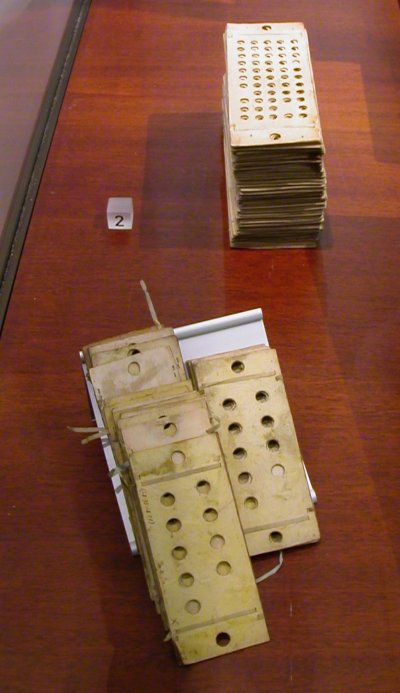
\includegraphics[scale=0.8]{images/misc/analytical_engine_punch_cards.jpg}
        \caption{Punch cards used to program the machine\\\tiny{Photo by Karoly Lorentey, sourced from wikimedia commons, under  Creative Commons Attribution 2.0 Generic license.}}
    \end{wrapfigure}

    As was mentioned before, Difference Engine project did end up exceeding given funding. Charles Babbage wasn't able to continue to work on his machine --- he couldn't
    afford his chief engineer in the project, Joseph Clement\footnote{Clement did end up owning all work he've done to himself, leaving Babbage virtually empty-handed}.
    This has lead Babbage to attempt an even more ambitious project in 1834 --- \emph{Analytical Engine}. While working on the Difference Engine, Babbage began to imagine
    ways of improving it, for it to support other kinds of calculations. Analytical Engine was something, we could call a computer in a general sense. It could be
    automated to perform any calculation set before it programmatically\footnote{\href{https://www.britannica.com/technology/Analytical-Engine}
    {https://www.britannica.com/technology/Analytical-Engine}}. I'm jumping a little bit forward here, but \emph{in the Babbage's lifetime, only a small trial 
    engine was constructed.}  \par


    Analytical Engine was designed to consist of four major elements: the mill, the store, the reader and the printer. Functionally, modern computers pretty much
    repeat this architecture. Those elements have very much resemblance with somewhat modern computer architectures. In this architecture, the mill acts as a `brain'
    of analytical engine, performing mathematical computations. The store was a place, where computer would hold it's data prior to computation. The reader and printer
    were an input and output units --- to `communicate' with an outside world, allowing to consume and output information. All computers now pretty much have the same 
    components functionally. If we are talking in informatics term, these components show strong resemblance to von Neumann architecture, described in 1945(!), more than
    100 years later. \par

    So, that's where an inspiration from Joseph Jacquard really kicks in! The principle behind punch cards, used in Jacquard Loom was adapted by Babbage to input data
    into his computer! It seems, that Babbage deeply respected Jacquard, having his woven portrait (with the help of Jacquard Loom, of course) in his 
    posession with at least \num{24000} punch cards used to create it\footnote{\href{https://www.sciencehistory.org/distillations/magazine/the-french-connection}
    {https://www.sciencehistory.org/distillations/magazine/the-french-connection}}. \par

    So, operating with those cards would give to one an ability to code necessary instructions for Analytical Engine to follow. Having a \emph{store} component, 
    where commands could be held before processing gave an ability to perform operations \emph{out of order}. In other words, computer was able not to just blindly
    follow commands punched on those cards, one by one, but rather have some `jumping' around in case of necessity. This opens a whole new level of controlling the
    program `flow', allowing for complex behaviour, based on meeting some criteria. `If that then do this' kind of stuff. Just to note, this feature was missing
    in many of the early computers of the 20\textsuperscript{th} century\footnote{\href{https://www.britannica.com/technology/Analytical-Engine}
    {https://www.britannica.com/technology/Analytical-Engine}}! \par

    \subsection{Enchantress of Numbers and Italy's Prime-Minister}

    Using punch cards as a format of input data not only have fascinated Babbage, but Ada Byrone too. For the next ten years, after the aforementioned party, she
    did study almost daily, learning from Babbage all she could about the machine. In the meantime she married William King in 1835, thus making her Ada King. In 1838
    William King was made Earl of Lovelace, making Ada the Countess of Lovelace. \emph{She mostly remembered by the name Ada Lovelace}. The two worked very closely,
    corresponding on the regular basis. \par

    Babbage gave lectures about his inventions sometimes. On one of such occasions he had a very special listener --- \emph{Luigi Federico Menabrea}, military student. Menabrea
    had quite a lot of achievements in his life: he later became engineer, doctor of mathematics, general, Count, Marquess of Valdora and seventh prime minister of Italy. 
    However, we are more interested in his academic publications. After learning about Babbage's Analytical Engine, he wrote a paper 
    `Notions sur la machine analytique de M. Charles Babbage'\footnote{\href{http://www.bibnum.education.fr/calcul-informatique/calcul/notions-sur-la-machine-analytique-de-m-charles-babbage}
    {http://www.bibnum.education.fr/calcul-informatique/calcul/notions-sur-la-machine-analytique-de-m-charles-babbage}} in which he, with great detail, described mathematical
    nuances regarding Babbage's machine. He also written it in French, as you could pick up from the title. \par

    Ada decided to translate Menabrea's work in English, titled `Sketch of the Analytical Engine invented by Charles Babbage'. Ada not only translated this publication, but
    also \emph{extended it with her own thought and commentary}. So, it became `Sketch of the Analytical Engine invented by Charles Babbage with Notes by the Translator Augusta Ada King, Countess Lovelace'.
    Her resulting work was published in 1843 and \emph{3 times as long as the original paper}\footnote{\href{https://www.historyofinformation.com/detail.php?id=467}{https://www.historyofinformation.com/detail.php?id=467}}. \par


    She also illustrated in her notes a sequential solution of various problems, through input in a form of punch cards into Analytical Engine. So, basically, she used 
    those punch cards the same way we are using keyboard and mouse to interact with the machine. Thus, making it the \emph{first ever documented and published program --- a 
    set of instructions for computer to follow}. So, meet the first programmer ever --- Countess Lovelace. \par

    % \begin{wrapfigure}{r}{0.5\textwidth}
    %     \centering
    %     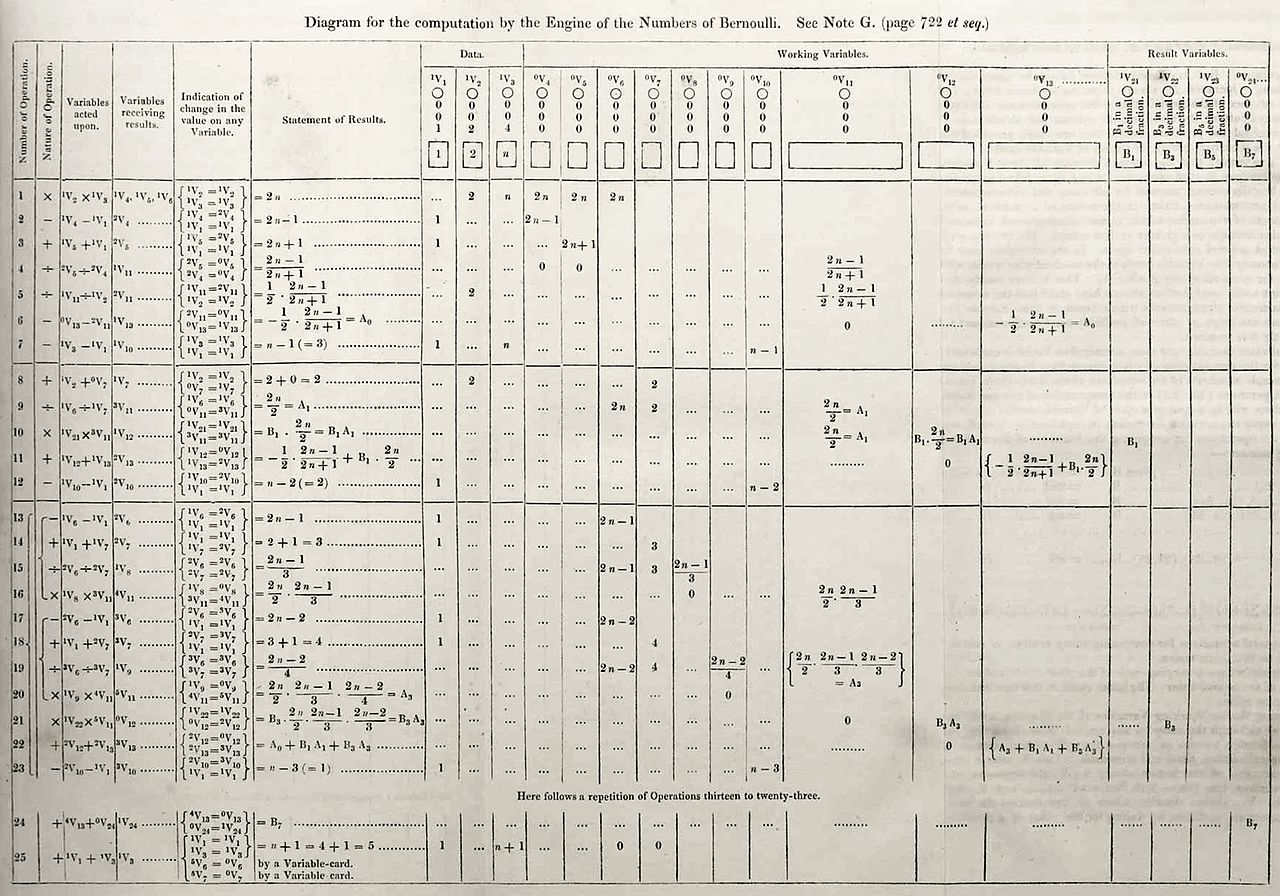
\includegraphics[scale=0.15]{images/misc/ada_lovelace_bernoulli_numbers_program.jpg}
    %     \caption{Program to calculate Bernoulli Numbers by Ada Lovelace}
    % \end{wrapfigure}


    \begin{wrapfigure}{l}{0.3\textwidth}
        \centering
        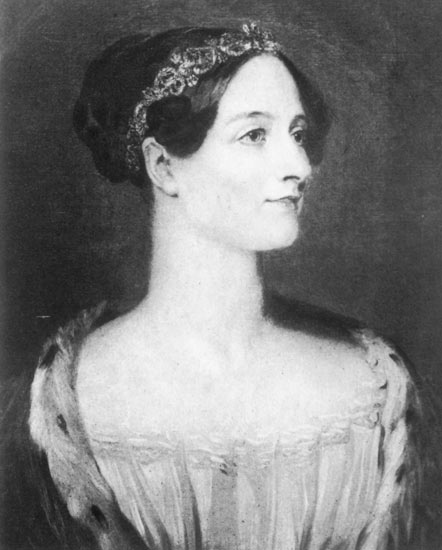
\includegraphics[scale=0.2]{images/persons/person_ada_lovelace.jpg}
        \caption{\\Augusta Ada King, \\ Countess of Lovelace}
    \end{wrapfigure}

    Although there are some disputes regarding the title of the `first programmer ever'\footnote{Most sources still say it is Ada Lovelace}, there is one thing virtually
    no one disputes: \emph{her understanding of the potential computers have}. Where Babbage have seen his own invention only crunching symbols and numbers, \emph{Ada saw
    potential to analyze and work with anything, provided there is a code for it, machine could understand}. In her notes for the translation, she wrote about objects besides
    numbers to be expressed by `science of operations' and gave an example of possibility for sounds to be expressed in such a way\footnote{\href{https://www.historyofinformation.com/detail.php?id=467}
    {https://www.historyofinformation.com/detail.php?id=467}}. Ada have also questioned computer's ability to `think on its own', and gave her thoughts on what will be later
    called \emph{artificial intelligence}\footnote{\href{https://medium.com/swlh/ada-lovelace-her-objection-e189717bd262}{https://medium.com/swlh/ada-lovelace-her-objection-e189717bd262}}.\par

    However, the history of Analytical Engine have ended due to a lack of funding, and it remained mostly on paper for the \emph{centuries} to come. Ada's late life 
    have taken a rather grim end, with lots of gambling, debts, opioid medications, adultery rumours and eventual death in 1852, 9 years after her first program and
    only in the of 36 years old\footnote{\href{https://www.biography.com/scholar/ada-lovelace}{https://www.biography.com/scholar/ada-lovelace}}. \par

    Charles Babbage continued to work on his machine until his death in 1871. As was said, machine was never finished in his lifetime.
    A version of his \emph{Difference Machine} without printing mechanism was built in 1991 by
    London Science Museum\footnote{\href{https://collection.sciencemuseumgroup.org.uk/objects/co526657/difference-engine-no-2-designed-by-charles-babbage-built-by-science-museum-difference-engine}
    {https://collection.sciencemuseumgroup.org.uk/objects/co526657/difference-engine-no-2-designed-by-charles-babbage-built-by-science-museum-difference-engine}}. 
    Constructors tried to adjust for physical properties achievable in 19\textsuperscript{th} century. It was concluded, that machine would've worked\footnote{\href{https://en.wikipedia.org/wiki/Difference_engine}
    {https://en.wikipedia.org/wiki/Difference\_engine}}. \par

    \subsection{Brief timeline of the computer history}

    Computer history is filled with many significant occasions since 19\textsuperscript{th} century. As was said, it is indeed a vast topic, although we will 
    mention few\footnote{Most occasions here are sourced from \href{https://www.computerhistory.org/timeline/}{https://www.computerhistory.org/timeline/}}:

    \begin{longtable}{p{0.2\textwidth}p{0.8\textwidth}}
        \toprule
        Year & Details \\
        \midrule
        1941 & Konrad Zuse finishes first programmable, electric digital computer, called Z3. Basically, all the Babbage wanted, 
                but with electricity in the form, we most familiar with, today\\
        \midrule
        1945 & John von Neumann described an architecture, that is the basis for virtually all of the computers we have today. 
                This architecture later will be known as `von Neumann Architecture' or `Architecture of von Neumann Machine'\\
        \midrule
        1948 & Claude Shannon formulated his first thoughts regarding what will be regarded as `Information Theory' in the future \\
        \cmidrule(r){2-2}
                & First computer program ran on the computer\\
        \midrule
        1952 & Grace Hopper invented first high-level programming language, A-0. It will evolve into COBOL later. \\
        \midrule
        1956 & Keyboard was succesfully connected to computer. Prior to this point, all programming had to be done by 
                punch cards or similar non-keyboard altertnatives\\
        \midrule
        1957 & FORTRAN created, \emph{first widely used high-level language}. \\
        \midrule
        1958 & LISP developed \\
        \midrule
        1960 & COBOL developed. COBOL \emph{still} highly in use today, especially in financial sector. Up to 80\% of the world's daily business transaction rely on 
        COBOL, source: \href{https://www.ibm.com/blogs/ibm-training/did-you-know-80-percent-of-the-worlds-daily-business-transactions-rely-on-cobol/}
        {https://www.ibm.com/blogs/ibm-training/did-you-know-80-percent-of-the-worlds-daily-business-transactions-rely-on-cobol/} \\

        \cmidrule(r){2-2}
                & ALGOL-60 developed \\
        \midrule
        1969 & ARPANET first online. ARPANET is a direct predecessor for the \emph{Internet} we know today\\
        \cmidrule(r){2-2}
                & Kenneth Thompson and Dennis Ritchie developed UNIX. It's not too much of a stretch to say, that it is one of the most significant OS in history
                of computers. They influenced virtually all OS in use today. Because of the UNIX, or with it heavy influence, we got Linux, iOS, OS X, Android and Windows\\
        \midrule
        1970 & First ATM can be used by general public. \\
        \cmidrule(r){2-2}
                & Pascal programming language developed. \\
        \midrule
        1972 & C language developed. C is one of the \emph{most influential} programming language there is. It's average popularity, by 
        TIOBE index, consistently ranked as \emph{top-2 since 1987}, source: \href{https://www.tiobe.com/tiobe-index/}{https://www.tiobe.com/tiobe-index/}.
        TIOBE index is a measure of programming languages, created and maintained by company of the same name in Netherlands. \\
        \midrule
        1973 & First handheld cellular mobile phone invented. Start of a mobile network we know today. \\
        \cmidrule(r){2-2}
            & First successful inter-network communications. Birth of the Internet as we know it today. \\ 
        \midrule
        1977 & Apple II computer is developed by Steve Wozniak and marketed by Steve Jobs. One of the first computers, intended for personal use. \\
        \cmidrule(r){2-2}
            & Atari video game console released. One of the first game consoles in history\\
        \midrule
        1978 & First Multi-User Domain games appeared. They allowed for multiple players play against each other. One of the first multiplayer competitive game experinces.\\
        \cmidrule(r){2-2}
            & First Computer Worm created.\\
        \midrule
        1983 & Internet officially launched \\
        \cmidrule(r){2-2}
            & Microsoft Word officially launched \\
        \midrule
        1985 & C\texttt{++} released \\
        \midrule
        1987 & Basic parameters for GSM standard agreed. GSM is the main standard used in mobile network today. \\
        \cmidrule(r){2-2}
            & Perl developed\\
        \midrule
        1990 & First commercially succesful Windows OS version released, Windows 3.0 \\
        \cmidrule(r){2-2}
            & Photoshop initially released \\
        \midrule
        1991 & Linus Torvalds released Linux kernel \\
        \cmidrule(r){2-2}
            & Charles Babbage's Difference Engine \#2 is constructed at London Museum. \\
        \midrule
        1993 & First online ads appeared \\
        \midrule
        1995 & Java 1.0 introduced \\
        \cmidrule(r){2-2}
            & Javascript released \\
        \midrule
        1999 & WiFi routers started to gain popularity for in-home usage. \\
        \midrule
        2000 & First mobile phone with camera released \\
        \cmidrule(r){2-2}
            & USB flash drives first apperaed on the market. \\
        \cmidrule(r){2-2}
            & Y2K problem. `Y2K' refers to potential computer errors related to the formatting and storage of calendar data. Not every program validly operated 
                with dates and there were many speculations about how this would affect computers.\\
        \midrule
        2004 & World of Warcraft comes on-line \\
        \cmidrule(r){2-2}
            & Google's IPO\\
        
        \bottomrule
        
        \caption{Some of significant occasions in computer history}
    \end{longtable}

    So, although this table cannot possibly reflect all significant events in the computer history, it demontsrates nicely how immensely far we've gone from the
    Babbage's steam-powered machines and Pascal's mechanical calculators. \par

    \subsection{History matters}

    I occasionally hear an argument about whether or not it is necessary to learn something as obscure as the history of computers and those weird looms and whatnot. The main
    reasoning of such argument being that it's not necessary to know history of programming to learn it. Although it might be true, nonetheless I don't only think it 
    wouldn't hurt too much to know it, I am sure that \emph{knowing such details could give a real insight to some technologies we use today}. Computer Science
    may not be the most ancient of sciences, but it does have it's history. It's not the history of the machines we are interested in, no. We are interested in 
    the history of the \emph{human thought}. It's not the machine that builds itself --- it's human's work. \emph{Any scientific and applicable discipline we know today
    is a result of accumulation of said thoughts}. \par

    Today we can see number of technologies, that emerged seemingly out of nowhere and dominated market, science, and 
    most importantly --- human minds. Just an example: blockchain and cryptocurrencies that today gracefully entered mainstream news and media were still a geeks'
    venue in early 2010s. But even if you knew about Bitcoin, in the year when Satoshi Nakamoto published his paper\footnote{\href{https://bitcoin.org/bitcoin.pdf}
    {https://bitcoin.org/bitcoin.pdf}}, did you knew, that blockchain was firstly described not in 2009, but in 
    1991(!)\footnote{\href{https://www.icaew.com/technical/technology/blockchain-and-cryptoassets/blockchain-articles/what-is-blockchain/history}
    {https://www.icaew.com/technical/technology/blockchain-and-cryptoassets/blockchain-articles/what-is-blockchain/history}}, 18 years before the notorius use case example
    in the face of the Bitcoin emerged? 18 years --- is a considerate time-span, especially in IT. In IT terms, to study such an old documents is the equivalent of
    archaeological studies\footnote{Maybe a bit of exaggeration, but you get the idea}. First works on the decentralised digital currency are emerged in 1998. Just to
    put it differently: \emph{in the end of the last century}, which is crazy to hear, talking about IT and something that entered mainstream today. \par

    Or we can see another example of the technology dominant today, which roots are deeply in the past: Artificial Intelligence and Machine Learning. Face recognitions, self-driving cars, fraud detections.
    AI and ML in some form or another is pretty much in the mainstream now. \emph{The field of artificial intelligence research was founded as an academic discipline in 1956}\footnote{
    \href{https://www.cantorsparadise.com/the-birthplace-of-ai-9ab7d4e5fb00?gi=a4c19646195c}{https://www.cantorsparadise.com/the-birthplace-of-ai-9ab7d4e5fb00?gi=a4c19646195c}}, around 66(!) years ago 
    from the moment I am writing this essay. It doen't sound like a bleeding edge of a technology now, eh\footnote{AI and ML has undoubtedly came a long way since then. Still though.}? \par

    Oftentimes what we call `modern' and `bleeding edge' is a simple reincarnation of old ideas. It's also not due to plagiarism or stealing, but simple practicality.
    Some concepts were just not implementable at the time of emerging. It mostly occurs due to hardware limitations. First self-driving car, using neural 
    networks\footnote{Technology imitating neurons in our brain, mostly used in ML and AI disciplines} was created in 1989\footnote{\href{https://neptune.ai/blog/self-driving-cars-with-convolutional-neural-networks-cnn}
    {https://neptune.ai/blog/self-driving-cars-with-convolutional-neural-networks-cnn}}. It was fairy simple by today's standards, but it served as a proof-of-concept,
    proving feasibility of further research. \par

    For us to delve in history --- is to understand motives and thoughts of our fellow curious minds. It helps us navigate and understand fundamental reasons of why
    something was made the way it was. Sometimes, revisiting old concepts can lead us to something new with the help of capabilities, provided by modern technologies.

\end{document}